% ============== Dark-Mode Skript mit bereinigten Boxen (XeLaTeX / LuaLaTeX) ==============
\documentclass[11pt,a4paper,oneside]{article}

% -------------------- Engine & Fonts --------------------
\usepackage{fontspec}
\setmainfont{Libertinus Serif}
\setsansfont{Libertinus Sans}
\usepackage{unicode-math}
\setmathfont{Libertinus Math}

% -------------------- Pakete --------------------
% --- Sprachen und Kodierung ---
\usepackage[ngerman]{babel}   % deutsche Sprachunterstützung
\usepackage{csquotes}         % korrekte Anführungszeichen

% --- Mathematik ---
\usepackage{amsmath}          % grundlegende Mathematikumgebung
\usepackage{mathtools}        % Erweiterungen für amsmath
\usepackage{physics}          % nützliche Makros für Physik
\usepackage{dsfont}           % Mengensymbole (z. B. \mathds{R})

% --- Schriften ---
% für XeLaTeX/LuaLaTeX: fontspec, unicode-math und Libertinus
\usepackage{fontspec}
\usepackage{unicode-math}
\setmainfont{Libertinus Serif}
\setsansfont{Libertinus Sans}
\setmonofont{Libertinus Mono}
\setmathfont{Libertinus Math}

% --- Layout und Typografie ---
\usepackage[top=3cm, bottom=3cm, left=2.5cm, right=2.5cm]{geometry}
\usepackage{microtype}        % schönerer Randausgleich
\usepackage[onehalfspacing]{setspace} % 1,5-facher Zeilenabstand
\usepackage{tocloft}          % Inhaltsverzeichnis anpassen
\renewcommand{\cftsecleader}{\cftdotfill{\cftdotsep}} 

% --- Farben und Boxen ---
\usepackage{xcolor}
\newcommand{\ricardo}[1]{%
	\colorbox{ForestGreen}{\color{white}\textsf{\textbf{Ricardo}}}%
	\textcolor{ForestGreen}{#1}%
}

% --- Tabellen und Listen ---
\usepackage{tabularx}
\usepackage{longtable}
\usepackage{dcolumn}
\usepackage{adjustbox}

% --- Grafiken ---
\usepackage{graphicx}
\usepackage{here}
\usepackage{floatflt}     % Bilder im Fließtext (eher alt)
\usepackage{epsfig}       % alte EPS-Unterstützung
\usepackage{epstopdf}     % Konvertierung EPS -> PDF

% --- Zitate und Literatur ---
\usepackage{cite}
\usepackage{bibgerm}      % deutsche BibTeX-Stile (alt; besser biblatex)

% --- Sonstiges ---
\usepackage{acro}         % Abkürzungsverzeichnis
\usepackage{blindtext}
\usepackage{lipsum}
\usepackage{listings}     % Quellcode
\usepackage{lettrine}     % Initialen
\usepackage[cute inductors,siunitx]{circuitikz} % Schaltpläne

\usepackage{pgfplots}
\pgfplotsset{compat=1.18} % aktuelle Version, sonst 1.17 oder 1.16
\usepackage{paralist}
\usepackage{tasks}
\usepackage{acro}
\usepackage{microtype}
\usepackage{geometry}
\usepackage{titlesec}
\usepackage{fancyhdr}
\usepackage{xcolor}
\usepackage{pagecolor}
\usepackage{tikz}
\usetikzlibrary{shadows,calc}
\usepackage[most]{tcolorbox}
\tcbuselibrary{skins,breakable,theorems}
\usepackage{enumitem}
\usepackage{caption}
\usepackage{everypage}
\usepackage{diagbox}
% -------------------- Layout --------------------
\geometry{
	left=28mm, right=28mm, top=28mm, bottom=28mm,
	marginparwidth=36mm, marginparsep=6mm
}

% -------------------- Farben (fein abgestuft, subtiler Fluss) --------------------
\definecolor{PageBG}{RGB}{17,11,31}             % sehr dunkler Hintergrund
\definecolor{TextCream}{RGB}{246,241,234}       % creme / sehr hell

\definecolor{AccentBlue}{RGB}{76,104,150}       % akademisches Blau (unverändert)
\definecolor{AccentViolet}{RGB}{105,77,145}     % seriöses Violett (unverändert)

% Hint: mehr ins violett/pinke ziehen (Hauch von Fuchsia)
\definecolor{AccentMagenta}{RGB}{140,60,120}       % violett-pink (sanfter Übergang)

% Magenta: rötlicher, dichter, aber nicht grell
\definecolor{AccentHint}{RGB}{170,40,60}     % rötliches Magenta (mehr Rotanteil)

% Elegantes Rot: orientiert sich am bisherigen "AccentHint" (tiefes Weinrot)
\definecolor{AccentRed}{RGB}{120,10,25}         % elegantes Weinrot / tiefes Rot

\definecolor{BoxBackground}{RGB}{15,9,27}       % Box-Hintergrund
\definecolor{MarginalGray}{RGB}{150,150,160}    % Rand-Datum

\pagecolor{PageBG}
\color{TextCream}


% -------------------- Kopf / Fuß --------------------
\pagestyle{fancy}
\fancyhf{}
\renewcommand{\headrulewidth}{0pt}
\setlength{\headheight}{14pt}
\fancyfoot[C]{%
	\vspace{6pt}%
	{\scriptsize\scshape Ferdinand-Braun Schule \quad • \quad Leistungskurs Mathematik Q3 \quad • \quad \thepage}%
	\begin{tikzpicture}[remember picture,overlay]
		\draw[line width=0.9pt,color=AccentViolet!80!black] ($(current page.south west)+(28mm,22mm)$) -- ($(current page.south east)+(-28mm,22mm)$);
	\end{tikzpicture}%
}

% -------------------- Titel-Styles --------------------
\titleformat{\section}
{\normalfont\large\bfseries\color{AccentBlue!33}}
{\thesection}
{1em}
{}
\titleformat{\subsection}{\normalfont\normalsize\bfseries\color{AccentViolet!33}}{\thesubsection}{0.8em}{}
\titleformat{\subsubsection}{\normalfont\normalsize\bfseries\color{AccentMagenta!33}}{\thesubsubsection}{0.6em}{}

% ========================= TCBOX BASIS-STIL (bereinigt) =========================
\tcbset{
	mybase/.style={
		enhanced,
		breakable,
		%drop shadow, 
		%shadow={1mm}{-1mm}{0mm}{black!50!white},
		boxrule=0.9pt,
		colframe=black!20,
		colback=BoxBackground,
		colupper=TextCream,          % Textfarbe innerhalb der Box
		arc=2mm,
		boxsep=5pt,
		left=15pt,right=15pt,top=15pt,bottom=15pt,
		before skip=8pt, after skip=8pt,
		attach boxed title to top left={yshift=-0.25mm-\tcboxedtitleheight/2, xshift=10mm},
		boxed title style={
			arc=4mm,
			left=6pt,right=6pt,top=3pt,bottom=3pt,
			boxrule=0pt           % kein zusätzlicher Rahmen für den Titelsticker
			% hier KEIN colback setzen — colbacktitle wird pro Box gesetzt
		},
		fonttitle=\sffamily\bfseries\small,
		title after break=\vspace{4pt}
	}
}

% -------------------- THEOREM (theo) --------------------
\newtcolorbox[auto counter,number within=section]{theo}[2][]{%
	mybase,
	colframe = AccentBlue!75!black,  %AccentViolet!75!black,
	colbacktitle = AccentBlue!85!black, %AccentViolet!85!black,
	coltitle = TextCream,
	title = {Theorem~\thetcbcounter: #2},
	#1
}

% -------------------- BEISPIEL (exem) --------------------
\newtcolorbox[auto counter,number within=section]{exem}[2][]{%
	mybase,
	colframe = AccentViolet!75!black, %AccentBlue!75!black,
	colbacktitle = AccentViolet!85!black,%AccentBlue!85!black,
	coltitle = TextCream,
	title = {Beispiel~\thetcbcounter: #2},
	#1
}

% -------------------- AUFGABE (aufgabe) --------------------
\newtcolorbox[auto counter,number within=section]{aufgabe}[2][]{%
	mybase,
	colframe = AccentMagenta!75!black, %AccentMagenta!75!black,
	colbacktitle = AccentMagenta!85!black, %AccentMagenta!85!black,
	coltitle = TextCream,
	title = {Aufgabe~\thetcbcounter: #2},
	#1
}

% -------------------- LÖSUNG (loesung) - zu Aufgabe passend --------------------
\newtcolorbox[use counter from=aufgabe]{loesung}[2][]{%
	mybase,
	colframe = AccentHint!75!black, %AccentMagenta!60!black,
	colbacktitle = AccentHint!85!black,%AccentMagenta!72!black,
	coltitle = TextCream,
	title = {Lösung~\thetcbcounter: #2},
	#1
}

% -------------------- Hinweis-Box --------------------
\newtcolorbox{infobox}[1][]{%
	mybase,
	colframe = AccentRed!75!black,
	colbacktitle = AccentRed!85!black,
	coltitle = TextCream,
	title = {Hinweis},
	#1
}

% ==================== Datum in rechter Margin (jede Seite) ====================
%\newcommand{\SetSideDateText}[1]{%
%	\gdef\@sidedatetext{#1}%
%	\AddEverypageHook{%
%		\begin{tikzpicture}[remember picture,overlay]
%			\node[anchor=north east,inner sep=0pt] at ($(current page.north east)+(-18mm,-14mm)$) {%
%				\parbox{32mm}{\raggedleft\small\sffamily\color{MarginalGray}\@sidedatetext}%
%			};
%		\end{tikzpicture}%
%	}%
%}
%\makeatletter \def\@sidedatetext{} \makeatother

% Makro für das Datum am rechten Rand
\newcommand{\lessondate}[1]{
	\noindent\hfill\textcolor{gray}{\textsc{#1}} \\
	\vspace{0.5cm}
}



% ==================== Feines Titelblatt ====================
\newcommand{\MakeArtTitle}[4]{%
	\begin{titlepage}
		\vspace*{18mm}
		\begin{center}
			%\begin{tikzpicture}
			%	\fill[AccentViolet!85!black] (0,0) circle (1.2cm);
			%	\fill[PageBG] (0.15,0.15) circle (0.95cm);
			%	\draw[line width=1pt,color=AccentBlue] (0,0) circle (1.35cm);
			%	\node[white] at (0,0) {\sffamily\bfseries\Large M};
			%\end{tikzpicture}
			\vspace{12mm}
			%{\Huge\bfseries\sffamily\color{TextCream} #1 \par}
			{\huge\color{TextCream} #1 \par}
			\vspace{6mm}
			{\Large\itshape\color{AccentBlue!50} #2 \par}
			\vspace{10mm}
			{\Large\scshape\color{TextCream} #3 \par}
			\vspace{6mm}
			{\small\color{MarginalGray} #4 \par}
			%\vfill
			\vspace{5mm}
			{\small\color{MarginalGray} \today \par}
			%\vspace{12mm}
			%\begin{tikzpicture}
			%	\draw[line width=1.2pt,color=AccentViolet!80!black] (-6,0) -- (6,0);
			%	\draw[line width=0.45pt,color=AccentBlue!60!black] (-6,-0.3) -- (6,-0.3);
			%\end{tikzpicture}
		\end{center}
		\vspace{7.5cm}
		\centering
		
\includegraphics[width=0.75\textwidth]{2.png} % Logo einfügen (Pfad anpassen)
	\end{titlepage}
}

% ==================== Dokumentbeginn ====================
\begin{document}
	
	% Titelblatt
	\MakeArtTitle{
		Leistungskurs Mathematik Q3 Hessen}
		{Stochastik Skript}
		{Shamsher Singh Kalsi}
		{Berufliches Gymnasium — Ferdinand-Braun Schule \\ Kursleiter: Herr Thorsten Farnungen}
	
	\tableofcontents
	\bigskip
	\clearpage
	
	
	\section{Einleitung}
	\lessondate{17.08.2025}\\
	Dieses Skript dient als Fortsetzung von der Q2. Hierbei werden nur thematisch theoretische Unterrichtsinhalte notiert, wobei die Aufgaben und Übungen hauptsächlich in Obsidian bearbeitet werden, um den wahnsinnigen Dokumentationsaufwand zu reduzieren. 
	
	\subsection{Leistungsbewertung und Klausurplanung in der Q3}
	\lessondate{20.08.2025}\\
	Im Verlauf des Schuljahres werden in diesem Kurs drei Klausuren geschrieben.
	Die zweite Klausur wird als Abiturklausur unter authentischen Bedingungen angesetzt, was eine Bearbeitungszeit von fünf Zeitstunden umfasst. Da der bis zu diesem Zeitpunkt behandelte abiturrelevante Stoff der Q3 ausschließlich die Stochastik abdeckt, wäre eine fünfstündige Prüfung allein zu diesem Thema für die Schülerinnen und Schüler eine unzumutbare Belastung. 
	Aus diesem Grund wird der hilfsmittelfreie Teil dieser Klausur auch Aufgaben aus den Qualifikationsphasen Q1 (Analysis) und Q2 (Analytische Geometrie/Lineare Algebra) beinhalten, um eine angemessene Themenbreite zu gewährleisten.
	Die erste Klausur ist für den Zeitraum vor den Herbstferien vorgesehen.
	
	\subsubsection{Randbemerkungen}

	%Zufallsexperimente, bei denen alle möglichen Ergebnisse \emph{gleich wahrscheinlich} angenommen werden. Dies ist kein naturwissenschaftliches Faktum, sondern ein mathematisches Modell unter Symmetrieannahmen.
	\begin{theo}{Laplace Experiment}
		Ein Zufallsexperiment mit endlicher Ergebnismenge $\Omega$ heißt
		\emph{Laplace-Experiment}, wenn für jedes Elementarereignis $\omega \in \Omega$
		gilt:
		\[
		P(\{\omega\}) = \frac{1}{|\Omega|}.
		\]
		Die Wahrscheinlichkeit eines Ereignisses $E \subseteq \Omega$ ist dann
		\[
		P(E) = \frac{|E|}{|\Omega|}.
		\]
	\end{theo}
	
	\begin{exem}
		Das Werfen eines idealen Würfels: $\Omega = \{1,2,3,4,5,6\}$,
		jedes Ergebnis hat Wahrscheinlichkeit $\tfrac{1}{6}$.
		Für das Ereignis $E=\{\text{gerade Zahl}\}$ gilt
		$P(E)=\tfrac{3}{6}=\tfrac{1}{2}$.
	\end{exem}
	
	\newpage
	
	\section{Grundlegende Begriffe der Stochastik}
	
	\begin{aufgabe}{Check in Kapitel 1}
		\begin{enumerate}
			\item Jan hat 20-mal in eine Lostrommel hineingegriffen und dabei 18 Nieten gezogen. 
			\begin{itemize}
				\item Berechnen Sie die relative Häufigkeit für den Gewinn als Bruch und in Prozent
				\item Jana erreichte bei 12 Ziehungen die Gewinnquote 25\%. Berechnen Sie die absolute und die relative Häufigkeit. 
			\end{itemize}
		\item Bei der Bundestagswahl 2013 haben sich $71.5\%$ der 62 Mio. Wahlberechtigten an der Wahl beteiligt. Die Stimmenverteilung für die einzelnen Parteien ist in Fig. 1 Dargstellt. 
		\begin{itemize}
			\item Geben Sie die Anteile der Stimmenverteilung als Bruch und Dezimalzahl an
			\item Berechnen Sie, wie groß der Stimmenanteil der einzelnen Parteien bezogen auf alle 62 Mio. Wahlberechtigten ist.
		\end{itemize}
		\item Begründen Sie welche Situation ein Laplace-Experiment darstellt
		\begin{itemize}
			\item Sie fragen einen Lehrer, an welchem Wochentag er sein Auto gewaschen hat 
			\item Sie ziehen ein Los aus einem Loseimer mit 120 Losen 
			\item Sie beobachten, ob der nächste Plattfuß an iuhrem Fahrrad vorne oder hinten auftritt
		\end{itemize}
		\item Berechnen Sie den Mittelwert der folgenden Zahlen: \\
		$2,5 \qquad 6,3 \qquad 1,9 \qquad 10, 0 \qquad 2,8 \qquad 5,6 \qquad 5,1 \qquad 7,8$
		\end{enumerate}
	\end{aufgabe}
	
	\newpage
	
	\begin{loesung}{}
		\subsection*{Aufgabe 1}
		\begin{align*}
			h = \frac{H}{n}, &\qquad n = 20, \qquad H = 20 - 18 = 2 \\
			h  &= \frac{2}{20} = \boxed{ \frac{1}{10} = 0.1 = 10\%}
		\end{align*}
		Jana's relative häufige Gewinnquote Beträgt $25\%$, sodass $75\% \lor \frac{3}{4}$ Nieten sein müssen. Es gilt; 
		\[
		h_n(A) = \frac{H_n(A)}{n},
		\]
		wobei $h_n(A)$ die relative und $H_n(A)$ die absolute Häufigkeit sind. 
		\begin{align*}
			H &= h \cdot n\\
			H &= \boxed{0.25 \cdot 12 = 3}  
		\end{align*}
		\subsection*{Aufgabe 2}		
		\subsubsection*{Stimmenverteilung}
		\begin{inparaitem}
			\item [\textbf{CDU}] : 34.1 \% $= \frac{34.1}{100} = 0.341$ |
			\item [\textbf{CSU}] : 7.4\% $= \frac{7.4}{100} = 0.074$ |
			\item [\textbf{SPD}] : 25.7 \% $= \frac{25.7}{100} = 0.257$ |
			\item [\textbf{FDP}] : 4.8\% $= \frac{4,8}{100} = 0.048$ |
			\item [\textbf{Die Linke}] : 8.6\%  $= \frac{8.6}{100} = 0.086$ |
			\item [\textbf{Die Grünen}] : 8.4\% $= \frac{8.4}{100} = 0.084$ |
			\item [\textbf{sonstige}] : 10.9 \%$= \frac{10.9}{100} = 0.109$ |
		\end{inparaitem}\\ 
		\subsubsection*{Stimmenanteil}
		\[
		\text{Wähler} = 62.000.000 \cdot 0.715 = 44.330.000
		\]
		\begin{itemize}[leftmargin= 4cm, font=\bfseries]
			\item [\textbf{CDU}] : 34.1 \% $= 0.341 \cdot 44.330.000 \approx \boxed{15.112.000}$ 
			\item [\textbf{CSU}] : 7.4\% $= 0.074 \cdot 44.330.000 \approx \boxed{3.280.420} $ 
			\item [\textbf{SPD}] : 25.7 \% $= 0.257 \cdot 44.330.000 \approx \boxed{11.392.810}$ 
			\item [\textbf{FDP}] : 4.8\% $= 0.048 \cdot 44.330.000 \approx \boxed{2.127.840}$ 
			\item [\textbf{Linke}] : 8.6\%  $=0.086 \cdot 44.330.000 \approx \boxed{3.812.380}$ 
			\item [\textbf{Grünen}] : 8.4\% $= 0.084 \cdot 44.330.000 \approx \boxed{3.723.720}$ 
			\item [\textbf{sonstige}] : 10.9 \%$= 0.109 \cdot 44.330.000 \approx \boxed{4.831.970}$ 
		\end{itemize}		
	\end{loesung}
	
	\newpage
	
	\begin{loesung}{}
		\subsection*{Aufgabe 3}
		\begin{enumerate}
			\item Kein Laplace-Experiment, da der Lehrer nicht mit gleicher Wahrscheinlichkeit an jedem Wochentag sein Auto wäscht; Alltagsroutinen und äußere Zwänge machen die Wahrscheinlichkeiten ungleich.
			\item Laplace-Experiment: Jedes der 120 Lose ist gleich wahrscheinlich gezogen zu werden, sofern alle Lose gleich beschaffen und gut gemischt sind. Dass die Gewinnchancen inhaltlich ungleich verteilt sind (1 Gewinnlos, 119 Nieten), widerspricht dem Laplace-Modell nicht, da sich dieses nur auf die Elementarereignisse (jedes einzelne Los) bezieht.
			\item Kein sauberes Laplace-Experiment, da das Vorderrad physikalisch häufiger betroffen ist (führt, trifft zuerst Hindernisse, andere Belastung). Nur unter starker Modellannahme „beide Räder gleich gefährdet“ könnte man es als Laplace-Experiment ansehen.
		\end{enumerate}
		\subsection*{Aufgabe 4}
		\begin{itemize}
			\item $2 + 5 = 7, \frac{7}{2} = 3,5$
			\item $6 + 3 = 9, \frac{9}{2} = 4.5$
			\item $1 + 9 = 10, \frac{10}{2} = 5$
			\item $10 + 0 = 10, \frac{10}{2} = 5$
			\item $2 + 8 = 10, \frac{10}{2} = 5$
			\item $5 + 6 = 11, \frac{11}{2} = 5.5$
			\item $5 + 1 = 6, \frac{6}{2} = 3$
			\item $7 + 8 = 15, \frac{15}{2}$
		\end{itemize}
		
		\textbf{Oder:} Um den Mittelwert (das arithmetische Mittel) $\bar{x}$ zu berechnen, werden alle Zahlen summiert und die Summe wird durch die Anzahl der Zahlen geteilt.
		\begin{align*}
			\bar{x} &= \frac{2,5 + 6,3 + 1,9 + 10,0 + 2,8 + 5,6 + 5,1 + 7,8}{8} \\
			\bar{x} &= \frac{42,0}{8} \\
			\bar{x} &= \boxed{5,25}
		\end{align*}
	\end{loesung}
	
	\newpage 
	\lessondate{25.08.2025}\\
	
	\begin{aufgabe}{Bearbeiten Sie die Aufgaben 1 bis 4 von Wdh. Statistik}
		\begin{enumerate}
			\item Berechnen Sie den Mittelwert, die Varianz und die Standardabweichung der Liste ${2; 0; 5; 6; 3; 8}$
			\item Von einer Lieferung Fahrradspeichen wurde bei einer Stichprobe die Länge der Speichen (in mm) gemessen: ${269; 274; 269; 268; 272; 270; 269; 270; 268; 271}$. 
			\begin{itemize}
				\item Nenne Sie die bei dieser Erhebung die Grundgesamtheit, den Mermalsträger, das untersuchte Merkmal, den Stichprobenumfang und die Merkmalsausprägungen. 
				\item Berechnen Sie den Mittelwert, die Varianz und die Standardabweichung 
			\end{itemize}
			\item Die Anzahl der Regentage beträgt im langjährigen Mittel für Amsterdam bzw. Rangun: 
			\begin{itemize}
				\item Stellen Sie die Verteilung der Anzahl der Regentage grafisch dar. 
				\item Berechnen Sie für beide Messreihen den Mittelwert und die Standartabweichung
			\end{itemize}
			\item Gegeben ist die nebenstehende relative Häufgikeitsveteilung.
			\begin{itemize}
				\item Beschriften Sie die Achsen passend 
				\item Bestimmen Sie den Mittelwert und die Standardabwichung 
				\item Untersuchen Sie, welche Werte aus b) sich ändern, wenn alle Säulen gleich hoch sind
			\end{itemize}
		\end{enumerate}
	\end{aufgabe}
	
	\newpage
	
	\begin{theo}{Die Bedeutung von Mittelwert, Varianz und Standardabweichung}
		\subsection*{Mittelwert}
		Der Mittelwert gibt sozusagen den Durchschnitt gegebener Daten an. Diesen Berechnet man durch das Addieren aller Elemente und dem Teilen von der Anzahl der Elemente. 
		\[
		\overline{x} = \frac{1}{n} \sum^{n}_{i = 1} x_i 
		\]
		\subsection*{Varianz}
		Die Varianz misst, wie stark die Werte um den Mittelwert streuen. Dazu berechnet man die Abweichungen jedes Wertes vom Mittelwert, quadriert diese (damit Abweichungen nach oben und unten nicht wegfallen) und mittelt sie wieder:
		\[
		s^2 = \frac{1}{n} \sum^{n}_{i = 1} (x_i - \overline{x})^2 
		\]
		\subsection*{Standardabweichung}
		Die Standardabweichung ist die Wurzel der Varianz. Sie gibt die Streuung in derselben Einheit wie die Daten an (praktischer als die quadrierten Werte der Varianz):
		\[
		s = \sqrt{s^2}
		\]
	\end{theo}
	
	\begin{loesung}{Aufgabe 1}
	\begin{enumerate}
		\item \subsection*{Mittelwert}
		\vspace{-4mm}
		\[
			\overline{x} = \frac{2 + 0 + 5 + 6 + 3 + 8}{6} = \boxed{\frac{24}{6} = 4}
		\]
		\item \subsection*{Varianz}
		\vspace{-6mm}
		\begin{align*}
			s^2 &= \frac{1}{n} \sum^{n}_{i = 1} (x_i - \overline{x})^2 = \frac{\sum^{n}_{i = 1} (x_i - \overline{x})^2}{n}\\
			&= \frac{(2 - 4)^2 + (0 - 4)^2 + (5 - 4)^2 + (6 - 4)^2 + (3 - 4)^2 + (8 - 4)^2}{6}\\
			&= \frac{4 + 16 + 1 + 4 + 1 + 16}{6} = \boxed{\frac{42}{6} = 7}
		\end{align*}
	\item \subsection*{Standardabweichung} 
	\[
	s = \sqrt{s^2} \rightarrow \boxed{\sqrt{7} \approx 2.65}
	\]
	\end{enumerate}
	\end{loesung}
	
	\newpage
	
	\begin{loesung}{Aufgabe 2}
		\begin{enumerate}
			\item \subsection*{Aufgabe A}
			\begin{itemize}[left=4cm]
				\item[\textbf{Grundgesamtheit:}] Alle Fahrradspeichen in der gesamten Lieferung 
				\item[\textbf{Merkmalsträger:}] Eine einzelne Fahrradspeiche 
				\item[\textbf{Merkmal:}] Die Länge der Speiche in mm 
				\item[\textbf{Stichprobenumfang:}] Es wurden 10 Speichen gemessen $\rightarrow n = 10$ 
				\item[\textbf{Merkmalausprägungen:}] ${269; 274; 269; 268; 272; 270; 269; 270; 268; 271}$
			\end{itemize}
			
			\item \subsection*{Aufgabe B}
			
			\subsubsection*{Mittelwert}
			\vspace{-4mm}
			\[
			\overline{x} = \frac{269 + 274 + 269 + 268 + 272 + 270 + 269 + 270 + 268 + 271}{10} 
			= \boxed{\frac{2700}{10} = 270}
			\]
			
			\subsubsection*{Varianz}
			\vspace{-6mm}
			\begin{align*}
				s^2 &= \frac{1}{n} \sum^{n}_{i = 1} (x_i - \overline{x})^2 \\[2mm]
				&= \frac{(269-270)^2 + (274-270)^2 + (269-270)^2 + (268-270)^2 + (272-270)^2}{10} \\
				&\quad + \frac{(270-270)^2 + (269-270)^2 + (270-270)^2 + (268-270)^2 + (271-270)^2}{10} \\[2mm]
				&= \frac{1 + 16 + 1 + 4 + 4 + 0 + 1 + 0 + 4 + 1}{10} \\[2mm]
				&= \boxed{\frac{32}{10} = 3.2}
			\end{align*}
			
			\subsubsection*{Standardabweichung}
			\[
			s = \sqrt{s^2} = \sqrt{3.2} \approx \boxed{1.79}
			\]
			
		\end{enumerate}
	\end{loesung}
	
	\newpage
	
	\begin{loesung}{Aufgabe 3}
    \subsection{Aufgabe A}
		\resizebox{\textwidth}{!}{
			\begin{tabular}{|c|c|c|c|c|c|c|c|c|c|c|c|c|}
				\hline
				Monat & Jan. & Feb. & März & April & Mai & Juni & Juli & Aug. & Sept. & Okt. & Nov. & Dez. \\
				\hline
				Amsterdam & 10 & 8 & 11 & 8 & 9 & 9 & 11 & 11 & 10 &13  & 11 & 11 \\
				\hline
				Rangun & 1 & 1 & 1 & 2 & 13 & 23 & 25 & 24 & 20 & 11 & 4 & 1 \\
				\hline
			\end{tabular}
		}
		
	\vspace{1cm}
	
	\begin{center}
		\begin{tikzpicture}
			\begin{axis}[
				width=\textwidth,
				height=8cm,
				ybar=0.4,
				bar width=8pt,
				enlarge x limits=0.1,
				ylabel={Regentage},
				xlabel={Monat},
				xtick=data,
				xticklabels={Jan,Feb,März,Apr,Mai,Juni,Juli,Aug,Sept,Okt,Nov,Dez},
				legend style={at={(0.5,-0.15)}, anchor=north, legend columns=-1}
				]
				\addplot[fill=blue!70!black] coordinates {(1,10) (2,8) (3,11) (4,8) (5,9) (6,9) (7,11) (8,11) (9,10) (10,13) (11,11) (12,11)};
				\addplot[fill=red!70!black]  coordinates {(1,1) (2,1) (3,1) (4,2) (5,13) (6,23) (7,25) (8,24) (9,20) (10,11) (11,4) (12,1)};
				\legend{\color{black}Amsterdam, \color{black}Rangun}
			\end{axis}
		\end{tikzpicture}
	\end{center}
	
		\subsection{Aufgabe B}
			\noindent
			\begin{minipage}[t]{0.48\textwidth}
				\subsubsection*{Amsterdam}
				\vspace{-3mm}
				{
					\begin{align*}
						\overline{x}_A &= \tfrac{10 + 8 + 11 + 8 + 9 + 9 + 11 + 11 + 10 + 13 + 11 + 11}{12} \\
						&= \boxed{\tfrac{122}{12} \approx 10.17}
					\end{align*}
				}
				{\footnotesize % unwichtige Zwischenschritte kleiner
					\begin{align*}
						s_A^2 &= \frac{1}{12}\sum_{i=1}^{12}(x_i-\overline{x}_A)^2 \\
						&= \frac{(10-10.17)^2 + (8-10.17)^2 + \dots + (11-10.17)^2}{12} \\
						&= \frac{24.67}{12} \approx \boxed{2.06}
					\end{align*}
				}% Ende footnotesize
				\[
				s_A = \sqrt{s_A^2} = \boxed{\sqrt{2.06}\approx 1.43}
				\]
			\end{minipage}\hfill
			\begin{minipage}[t]{0.48\textwidth}
				\subsubsection*{Rangun}
				\vspace{-3mm}
				{\footnotesize
				\begin{align*}
					\overline{x}_R &= \frac{1 + 1 + 1 + 2 + 13 + 23 + 25 + 24 + 20 + 11 + 4 + 1}{12} \\
					&= \boxed{\tfrac{126}{12} = 10.5}
				\end{align*}
				}
				{\footnotesize
					\begin{align*}
						s_R^2 &= \frac{1}{12}\sum_{i=1}^{12}(x_i-\overline{x}_R)^2 \\
						&= \frac{(1-10.5)^2 + (1-10.5)^2 + \dots + (1-10.5)^2}{12} \\
						&= \frac{971}{12} \approx \boxed{80.92}
					\end{align*}
				}
				\[
				s_R = \sqrt{s_R^2} = \boxed{\sqrt{80.92}\approx 8.99}
				\]
			\end{minipage}
	\end{loesung}
	
	\newpage
	
	\begin{loesung}{Aufgabe 4}
		\subsection*{1. Achsenbeschriftung}
		\begin{itemize}
			\item X-Achse: „Merkmal“ bzw. „Anzahl Ereignisse“
			\item Y-Achse: „Relative Häufigkeit [\%]“
			\item Skalierung: $0 \%$ bis $40 \%$ in $10 \%$-Schritten
		\end{itemize}
		
		\subsection*{2. Mittelwert und Standardabweichung}
		
		Gegeben:
		\[
		x_i = 0,1,2,3, \qquad f_i = 0.1,0.2,0.3,0.4
		\]
		
		\paragraph{Mittelwert:}
		\[
		\overline{x} = \sum_i x_i \cdot f_i 
		= 0\cdot 0.1 + 1\cdot 0.2 + 2\cdot 0.3 + 3\cdot 0.4
		= 2.0
		\]
		
		\paragraph{Varianz:}
		\[
		s^2 = \sum_i f_i \cdot (x_i - \overline{x})^2
		= 0.1\cdot (0-2)^2 + 0.2\cdot (1-2)^2 + 0.3\cdot (2-2)^2 + 0.4\cdot (3-2)^2
		= 1.0
		\]
		
		\paragraph{Standardabweichung:}
		\[
		s = \sqrt{1.0} = 1.0
		\]
		
		\subsection*{3. Gleich hohe Säulen}
		
		Falls alle $f_i = 0.25$ gilt:
		
		\paragraph{Mittelwert:}
		\[
		\overline{x} = 0\cdot0.25 + 1\cdot0.25 + 2\cdot0.25 + 3\cdot0.25 = 1.5
		\]
		
		\paragraph{Varianz:}
		\[
		s^2 = 0.25\cdot(0-1.5)^2 + 0.25\cdot(1-1.5)^2 
		+ 0.25\cdot(2-1.5)^2 + 0.25\cdot(3-1.5)^2 = 1.25
		\]
		
		\paragraph{Standardabweichung:}
		\[
		s = \sqrt{1.25} \approx 1.118
		\]
	\end{loesung}
	
	
	\newpage

	
	\section{Berechnung von Wahrscheinlichkeiten}
	
	\lessondate{25.08.2025}\\
	
	\begin{theo}{Ereignis}
		Mathematisch gesehen ist ein Ereignis E also nichts anderes als eine Teilmenge des Ergebnisraumes $\Omega: E \subseteq  \Omega$
	\end{theo}
	
	\subsection{Boolische Algebra - Elemente der Mengenlehre}
	
	Buch Seite 32/33 Übung 4, 5 und 6 / Altes Buch Seite 12
	
	\begin{aufgabe}{Altes Buch Seite 12 Aufgaben 4, 5 und 6}
		\begin{itemize}
			\item [Übung 4] EIn Würfel wird einmal geworfen. Stellen Sie die Ereignisse $F_1:$ "Die Augenzahl ist kleiner als 3" und $E_2:$ "Die Augenzahl ist ungerade " als Ergebnismengen dar. Bestimmen Sie die Ergebnissmenge des Ereignisses $E_1 \cup E_2$
			\item [Übung 5] Aus einer Urne mit 50 gleichartigen Kugeln, die die Nummern 1 bis 50 tragen, wird zufällig eine Kugel gezogen. Stellen Sie die folgenden Ereignisse als Ergebnissmengen dar
			\item [Übung 6] Stellen Sie die folgenden Eregnisse beim Roulette als Ergebnismengen dar:  
		\end{itemize}
	\end{aufgabe}
	
	\begin{loesung}{Übung 5}
		\begin{itemize}
			\item $E_1 = 9, 18, 27, 36, 45$ 
			\item $E_2 = 12, 24, 36, 48$
			\item $E_3 = 23, 46$
		\end{itemize}
		\begin{align*}
			E_1 \cap E_2 &= \{36\}\\
			E_1 \cup E_2 &= \{9, 12, 18, 24, 27, 36, 45, 48\}\\
			E_2 \cap E_3 &= \{\}\\
			E_1 \cup E_2 \cup E_3 &= 
		\end{align*}
	\end{loesung}
	
	\newpage
	
	\begin{aufgabe}{Aufgabe 8 Ergebnismengen}
		EIn grüner und ein roter Würfel werden gleichzeitig geworfen. 
		\begin{itemize}
			\item Geben Sie einen Ergebnisraum an. Schreiben Sie hierzu ein Ergebnis als Paar.
			\item Geben Sie die Ergebnismenge folgender Ergebnisse an: 
			\begin{itemize}
				\item $E_1:$ Die Augenzahlen der beiden Würfel sind gleich 
				\item $E_2:$ Die Augensumme beträgt 8 
				\item $E_3:$ Das Augenzahlprodukt ist durch 8 teilbar 
				\item $E_4:$ Die Augenzahlen sind nicht beide gerade 
				\item $E_5:$ Das Produkt der Augenzahlen ist größer als 10, aber kleiner als 21
				\item $E_6:$ Die Augenzahlen unterscheiden sich um maximal 3
				\item $E_1 \cap E_2$
				\item $E_1 \cup E_2$
			\end{itemize}
		\end{itemize}
	\end{aufgabe}
	
	\begin{loesung}{Aufgabe 8}
		\begin{itemize}
			\item $\Omega := E_1 \cross E_2$
			\item 
		\end{itemize}
	\end{loesung}
	
	\newpage
	
	\subsection{Absolute und Relative Häufigkeit}
	
	\subsubsection{Relative Häufigkeit}
	
	\begin{aufgabe}{Übungen relative Häufigkeiten}
		\begin{itemize}[left=15mm]
			\item [Aufgabe 4]
			\item [Aufgabe 5]
			\item [Aufgabe 6]
			\item [Aufgabe 7]
			\item [Aufgabe 8]
		\end{itemize}
	\end{aufgabe}
	
	\begin{loesung}{Aufgabe 4}
		Das Würfeln wurde mithilfe eines Programmcodes simuliert. 
		Dabei ergaben sich die in Abbildung \ref{fig:wuerfel} dargestellten Resultate.
		%\begin{figure}[h!]
			\centering
			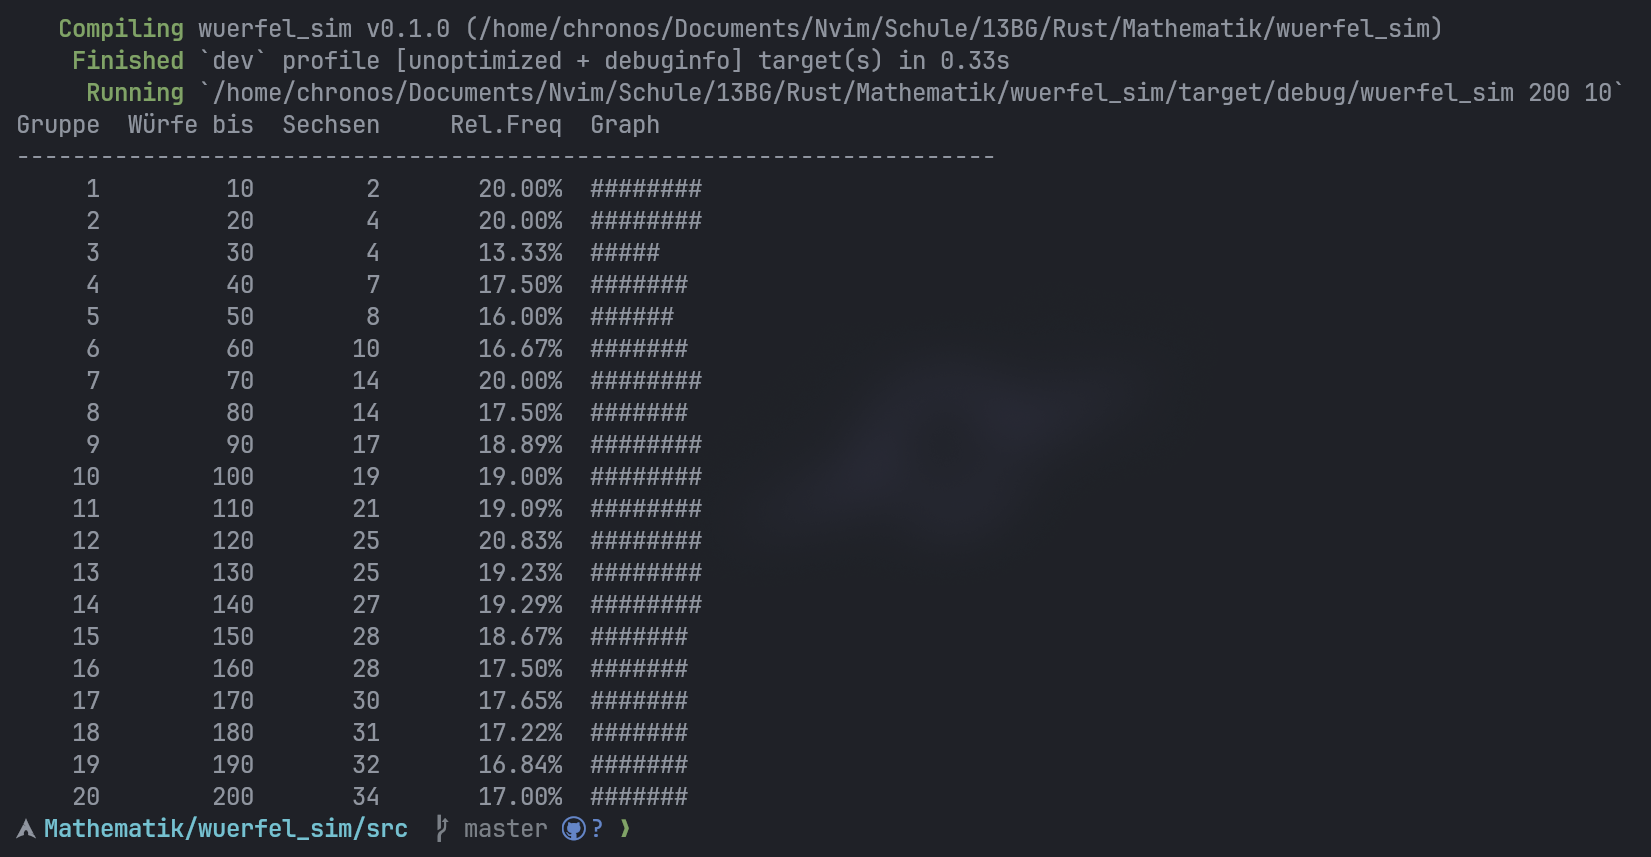
\includegraphics[width=\textwidth]{wuerfel.png}
			%\caption{Simulation der Würfelergebnisse}
			\label{fig:wuerfel}
		%\end{figure}
		\footnote{Unfertiger Code zur Vereinfachung}
	\end{loesung}
	
	\newpage
	
	\subsection{Laplace Wahrscheinlichkeit}
	
	\lessondate{27.08.2025}\\
	
	\begin{theo}{Satz: Wahrscheinlichkeiten bei Laplace Experimenten}
		Bei einem Laplace-Experiment sei \(\Omega = \{e_{1}, \dots, e_{m}\}\) der Ergebnisraum und \(E = \{e_{i_1}, \dots, e_{i_k}\}
		\) ein beliebiges Ereignis: Dann gilt für die Wahrscheinlichkeit deieses Ergebnisses; 
		\[
		P(E) =  \frac{|E|}{\Omega} =  \frac{k}{m} \qquad P(E) = \frac{\text{Anzahl der für E günstigen Ergebnisse}}{\text{Anzahl aller möglichen Ergebnisse}}
		\] 
	\end{theo}
	
	\begin{exem}
		content...
	\end{exem}
	
	\begin{aufgabe}{Aufgaben 9 bis 11}
		\begin{itemize}
			\item 
		\end{itemize}
	\end{aufgabe}
	
	\begin{loesung}{Aufgabe 9}
		Urne 2
	\end{loesung}
	
	\begin{loesung}{Aufgabe 10}
		\begin{enumerate}
			\item $\frac{1}{32}$
			\item $\frac{8}{32} = \frac{1}{4}$
			\item $P_L (E) = \frac{12}{32} \land P_H (E) = \frac{8}{32}$ 
		\end{enumerate}
	\end{loesung}
	
	\begin{loesung}{Aufgabe 11}
		\begin{enumerate}
			\item $\frac{4}{500}$
			\item $\frac{20}{500}$
			 \item $\frac{480}{500}$
			 \item 497 lose
		\end{enumerate}
	\end{loesung}
	
	
	\newpage
	
	Buch Seite 44 / 45 15 - 18
	
	\begin{aufgabe}{Buch Seite 45 Aufgaben 15 bis 18}
		content...
	\end{aufgabe}
	
	\begin{loesung}{Aufgabe 15}
		
		\begin{center}
			\begin{tabular}{|c|c|c|c|c|c|c|}
				\hline
				\diagbox{W1}{W2} & \color{red} 1 & \color{red} 2 & \color{red} 3  & \color{red} 4 & \color{red} 5 & \color{red} 6  \\ \hline
			    \color{red} 1 & 1& 2& 3 & 4 & 5 & 6 \\ \hline
				\color{red} 2 & 2 & 4 & 6 & 8 & 10 & 12 \\ \hline
				\color{red} 3 & 3 & 6 & 9 & 12 & 15 & 18 \\ \hline
				\color{red} 4 & 4 & 8 & 12 &  16& 20 & 24 \\ \hline
				\color{red} 5 & 5 & 10 & 15 & 20 & 25 & 30 \\ \hline
				\color{red} 6 & 6 & 12 & 18 & 24 & 30 & 36 \\ \hline
			\end{tabular}
		\end{center}
		\[
		\Omega = 36 
		\]
	\end{loesung}
	
	
	\newpage
	
	\lessondate{01.09.2025}\\
	
	\begin{aufgabe}{Übungen - Wahrscheinlichkeitsrechnung}
		\begin{enumerate}
			\item Berechnen Sie für die Urliste $\{4;3; 4; 5; 4 \}$ den Mittelwert, die Varianz und die Standardabweichung.
			\item Nach einer Statistik der Deutschen Bahn verkehren etwa 95 Prozent der Fernzüge „pünktlich (d.h. mit maximal 5 Minuten Verspätung). Tim fährt 5-mal mit einem Fernzug.
			\begin{itemize}
				\item Er berechnet die Wahrscheinlichkeit, dass mindestens ein Zug nicht pünktlich ist, mit der Formel $1 - 0.95^5$. Erklären Sie.
				\item Nehmen Sie Stellung zur Annahme: „Die Pünktlichkeit der Züge ist voneinander unabhängig."
			\end{itemize} 
		\item Wenn man Flügelmuttern auf einer Seite schwarz, auf der anderen weiß markiert, gibt es beim Würfeln drei mögliche Ergebnisse. Heiko hat 50-mal, Simon 200-mal gewürfelt.
		\begin{itemize}
			\item Notieren Sie sinnvolle Wahrscheinlichkeiten. Erläutern Sie Ihre Gedanken.
			\item Fassen Sie die Ergebnisse zusammen und notieren Sie eine bessere Einschätzung 
		\end{itemize}
		\item Man wirft zwei Würfel. Untersuchen Sie die Ereignisse A und B auf Unabhängigkeit. 
		\begin{itemize}
			\item A: Die Augensumme ist 6. Und B: Die Differenz der Augenzahl ist 0.
			\item A: Der erste Würfel zeigt 3. Und B: Die Augensumme ist größer als 5.
			\item A: Der erste Würfel zeigt eine Augenzahl unter 3. Und B: Der zweite Würfel zeigt einer Augenzahl über 3. 
		\end{itemize}
		\begin{center}
			\begin{tabular}{|c|c|c|c|}
				\hline 
				\diagbox{Namen}{Ergebnisse} & Schwarz & Weiß & Boden\\ \hline 
				Heiko & 20 & 24 & 6 \\ \hline
				Simon & 88 & 95 & 17 \\ \hline 
			\end{tabular}
		\end{center}
		\end{enumerate}
	\end{aufgabe}
	
	
	\newpage
	
	\begin{loesung}{Aufgabe 1}
		\subsection*{MIttelwert}
		\vspace{-10mm}
		\begin{align*}
			\overline{x} &= \frac{1}{n} \sum^{n}_{i = 1} x_i \\
			\overline{x} &= \frac{4 + 3 + 4 + 5 + 4 }{5} = \boxed{\frac{20}{5} = 4}
		\end{align*}
		\subsection*{Varianz}
		\vspace{-10mm}
		\begin{align*}
			s^2 &= \frac{1}{n} \sum_{i = 1}^{n} (x_i - \overline{x})^2 \\
			s^2 &= \frac{(4 - 4)^2 + (3 - 4)^2 + (4 - 4)^2 + (5 - 4)^2 + (4 - 4)^2}{5} \\
			s^2 &= \frac{0 + 1 + 0 + 1 + 0}{5} = \boxed{\frac{2}{5}  =0.4}
		\end{align*}
		\subsection*{Standardabweichung}
		\vspace{-10mm}
		\begin{align*}
			s &= \sqrt{s^2}\\
			s &= \sqrt{0.4} \approx \boxed{0.632} 
		\end{align*}
	\end{loesung}
	
	\begin{loesung}{Aufgabe 2}
		\subsection*{Erklärung zu $1-0{,}95^5$}
		Wir modellieren jede Fahrt als Bernoulli-Experiment mit der Erfolgswahrscheinlichkeit $p=0{,}95$ für „pünktlich“. Unter der (idealisierenden) Annahme stochastischer Unabhängigkeit ist die Wahrscheinlichkeit, dass \emph{alle} fünf Fahrten pünktlich sind, $0{,}95^5$. Das Gegenereignis lautet „mindestens eine Fahrt ist unpünktlich“, also $1-0{,}95^5\approx 1-0{,}77378094\approx 0{,}2262$.
		
		\subsection*{Zur Unabhängigkeits-Annahme}
		Die Annahme unabhängiger Fahrten ist eine bequeme Modellvereinfachung, aber in der Realität fragil: Systemstörungen, Wetterlagen, Bauarbeiten oder Anschlussabhängigkeiten erzeugen Korrelationen. Fahrten am selben Tag, auf derselben Strecke oder mit engen Umstiegsbeziehungen sind typischerweise positiv korreliert in ihrer Pünktlichkeit. Das Binomialmodell liefert also eine sinnvolle Erstnäherung; streng genommen wäre ein Modell mit latenten „Zuständen“ (z.\,B. normaler Betrieb vs. Störungstag) plausibler, bei dem sich $p$ zwischen Tagen variiert, sodass die Unabhängigkeit nur \emph{bedingt} gilt.
	\end{loesung}
	
	\begin{loesung}{Aufgabe 3}
		\subsection*{Gedanken zu sinnvollen Wahrscheinlichkeiten}
		Die Flügelmutter besitzt zwei markierte Flächen (schwarz/weiß), die geometrisch symmetrisch sind; hierfür ist ohne weitere Information $P(\text{Schwarz})\approx P(\text{Weiß})$ naheliegend. Ein Fall „Boden/Seite“ ist physikalisch möglich, aber aufgrund der kleineren stabilen Auflagefläche plausibel seltener als die Flächen. Eine uninformierte Vorabschätzung könnte also in der Größenordnung „je Flächenfarbe ähnlich groß, Boden merklich kleiner“ liegen, etwa symbolisch $P_S\approx P_W$ und $P_B$ deutlich darunter, ohne exakte Werte festzulegen.
		
		\subsection*{Schätzungen aus den Daten}
		Heiko würfelt $n_H=50$-mal mit $(20,24,6)$ für (Schwarz, Weiß, Boden), Simon $n_S=200$-mal mit $(88,95,17)$. Die relativen Häufigkeiten einzeln sind
		\[
		\hat p^{(H)}_S= \tfrac{20}{50}=0{,}40,\quad 
		\hat p^{(H)}_W= \tfrac{24}{50}=0{,}48,\quad
		\hat p^{(H)}_B= \tfrac{6}{50}=0{,}12,
		\]
		\[
		\hat p^{(S)}_S= \tfrac{88}{200}=0{,}44,\quad 
		\hat p^{(S)}_W= \tfrac{95}{200}=0{,}475,\quad
		\hat p^{(S)}_B= \tfrac{17}{200}=0{,}085.
		\]
		Fassen wir die Ergebnisse zusammen ($n=250$ Gesamtwürfe), erhalten wir
		\[
		\hat p_S=\frac{108}{250}=0{,}432,\qquad
		\hat p_W=\frac{119}{250}=0{,}476,\qquad
		\hat p_B=\frac{23}{250}=0{,}092.
		\]
		Diese gepoolte Schätzung ist robuster als die einzelne von Heiko, da $n$ größer ist. Sie bestätigt die Symmetrie zwischen den Flächen näherungsweise und zeigt einen kleineren, aber nicht vernachlässigbaren Anteil für „Boden“. Für weitere Präzision könnte man Konfidenzintervalle (z.\,B. Wilson) angeben; heuristisch liegt der Standardfehler pro Kategorie etwa bei $\sqrt{\hat p(1-\hat p)/n}$, also in einer Größenordnung von zwei bis drei Prozentpunkten für die Flächen und etwa zwei Prozentpunkten für „Boden“.
	\end{loesung}
	
	\begin{loesung}{Aufgabe 4}
		Es gelten $36$ gleichwahrscheinliche Ausgänge für zwei faire Würfel. Unabhängigkeit liegt genau dann vor, wenn $P(A\cap B)=P(A)\,P(B)$.
		
		\subsection*{A: Augensumme $=6$; B: Differenz $=0$}
		Die Summe $6$ tritt in $5$ Paaren auf, also $P(A)=\tfrac{5}{36}$. Die Differenz $0$ bedeutet gleiche Augen, also $P(B)=\tfrac{6}{36}=\tfrac{1}{6}$. Im Schnittpunkt liegt nur $(3,3)$, somit $P(A\cap B)=\tfrac{1}{36}$. Da 
		\[
		P(A)P(B)=\tfrac{5}{36}\cdot\tfrac{1}{6}=\tfrac{5}{216}\neq \tfrac{1}{36},
		\]
		sind $A$ und $B$ \emph{abhängig}.
		
		\subsection*{A: Erster Würfel zeigt $3$; B: Augensumme $>5$}
		Hier ist $P(A)=\tfrac{1}{6}$. Für $B$ gilt $P(B)=\tfrac{26}{36}=\tfrac{13}{18}$, da die Summen $\le 5$ insgesamt $1+2+3+4=10$ Fälle haben. Der Schnitt $A\cap B$ verlangt beim ersten Würfel $3$ und beim zweiten eine $3,4,5,6$, also $4$ von $36$: $P(A\cap B)=\tfrac{4}{36}=\tfrac{1}{9}$. Das Produkt
		\[
		P(A)P(B)=\tfrac{1}{6}\cdot \tfrac{13}{18}=\tfrac{13}{108}\neq \tfrac{1}{9},
		\]
		also \emph{abhängig}.
		
		\subsection*{A: Erster Würfel $<3$; B: Zweiter Würfel $>3$}
		Es ist $P(A)=\tfrac{2}{6}=\tfrac{1}{3}$ und $P(B)=\tfrac{3}{6}=\tfrac{1}{2}$. Der Schnitt umfasst die $2\cdot 3=6$ Paare mit erstem Wurf $1$ oder $2$ und zweitem Wurf $4,5,6$, also $P(A\cap B)=\tfrac{6}{36}=\tfrac{1}{6}$. Da
		\[
		P(A)P(B)=\tfrac{1}{3}\cdot \tfrac{1}{2}=\tfrac{1}{6},
		\]
		sind $A$ und $B$ \emph{unabhängig}.
	\end{loesung}
	
	\lessondate{05.09.2025}\\	
	
	\begin{aufgabe}{ Buch Seite 49 Mehrstufige Zufallsversuche}
		\begin{itemize}
			\item \textbf{Aufgabe 5:} In einer Schublade liegen fünf Sicherungen, von denen zwei defekt sind. Wie groß ist die Wahrscheinlichkeit, dass bei zufälliger Entnahme von zwei Sicherungen aus der Schublade mindestens eine defekte Sicherung entnommen wird? 
			\item \textbf{Aufgabe 7:} Das abgebildete Glücksrad (mit drei gleich gtoßen Sektoren) wird zweimal gedreht. Mit welcher Wahrscheinlichkeit
			\begin{itemize}
				\item erscheint in beiden Fällen rot, 
				\item erscheint mindestens einmal rot? 
			\end{itemize}
			\item \textbf{Aufgabe 9:}
			In einer Urne liegen 7 Buchstaben, viermal das "O" und dreimal das "T". Es werden vier Buchstaben der Reihe nach mit Zurücklegen gezogen. Mit welcher Wahrscheinlichkeit
			\begin{itemize}
				\item entsteht das Wort "OTTO"
				\item lässt sich mit den gezogenen Buchstaben das Wort "OTTO" bilden? 
			\end{itemize} 
		\end{itemize}
	\end{aufgabe}	
	
		\begin{aufgabe}{ Buch Seite 50 Mehrstufige Zufallsversuche}
		\begin{itemize}
			\item \textbf{Aufgabe 11:} Robinson hat festgestellt, dass auf seiner Insel folgende Wetterregeln gelten: Ist es schön, ist es morgen mit $80\%$ Wahrscheinlichkeit ebenfalls schön. Ist heute schlechtes Wetter, so ist morgen mit $75\%$ Wahrscheinlichkeit ebenfalls schlechtes Wetter. 
			\begin{itemize}
				\item Heute (Montag) scheint die Sonne. Mit welcher Wahrscheinlichkeit kann kann Robinson am Mittwoch mit schönem Wetter rechnen? 
				\item Heute ist Dienstag und es ist schön. Mit welcher Wahrscheinlichkeit regnet es am Freitag? 
			\end{itemize}
			\item \textbf{Aufgabe 14:} Die drei Räder eines Glücksautomaten sind jeweils in 5 gleich große Sektoren eingeteilt und drehen sich unabhängig voneinander (Abbildung - Erstes Rad bestehend aus; x, y, z, y, z - Zweites Rad bestehend aus; x, y, z, y, z - Drittes Rad bestehend aus; y, z, x, x, x).Die Einzahlung beträgt 0.50 Euro.
			\begin{itemize}
				\item x, x, x, = 7 Euro 
				\item y, x, y = 2 Euro
				\item y, z, y = 2 Euro 
				\item  y, y, y = 2 Euro 
			\end{itemize} 
			\begin{itemize}
				\item Mit welcher Wahrscheinlichkeit gewinnt $7$ Euro bzw. $2$ Euro? 
				\item Lohnt sich das Spiel auf langer sicht? 
			\end{itemize}
		\end{itemize}
	\end{aufgabe}
	
		\begin{aufgabe}{ Buch Seite 51 Mehrstufige Zufallsversuche}
		\begin{itemize}
			\item \textbf{Aufgabe 17:} Bei dem abgebildeten Glücksrad tritt jedes der 10 Felder mit der gleichen Wahrscheinlichkeit ein. Das Glücksrad wird zweimal gedreht. \{9,7,9,9,7,9,9,7,1,9\}
			\begin{itemize}
				\item Stellen Sie eine geeignete Ergebnismenge für dieses Zufallsexperiment  auf und geben Sie die Wahrscheinlichkeiten aller Elementarereignisse mit Hilfe eines Baumdiagrammes an. 
				\item Berechnen Sie die Wahrscheinlichkeiten der folgenden Ereignisse: 
				\begin{itemize}
					\item A: Es tritt höchstens einmal die 1 auf
					\item B: Es tritt genau einmal die 7 auf 
					\item C: Es tritt keine 9 auf 
					\item D = B $\cap$ C
				\end{itemize}
			\end{itemize}
		\end{itemize}
	\end{aufgabe}
	
	\begin{loesung}{Buch Seite 49 Mehrstufige Zufallsversuche}
		
		\subsection*{Aufgabe 5}
		In einer Schublade liegen 5 Sicherungen, davon 2 defekt und damit 3 intakt. Es werden ohne Zurücklegen zwei Sicherungen gezogen. Gesucht ist
		\[
		P(\text{mindestens eine defekt}) = 1 - P(\text{keine defekt}).
		\]
		Anzahl günstiger Fälle für ``keine defekt'': aus den 3 intakten Sicherungen werden 2 gewählt:
		\[
		\binom{3}{2}=3.
		\]
		Anzahl aller gleich wahrscheinlichen Ziehungen:
		\[
		\binom{5}{2}=10.
		\]
		Also
		\[
		P(\text{keine defekt})=\frac{3}{10},
		\]
		und damit
		\[
		P(\text{mindestens eine defekt})=1-\frac{3}{10}=\frac{7}{10}=0{,}7.
		\]
	\end{loesung}
	
	\begin{loesung}{}
		\subsection*{Aufgabe 7}
		Das Glücksrad hat drei gleich große Sektoren, davon sei genau einer rot. Bei zwei unabhängigen Drehungen gilt für die Eintrittswahrscheinlichkeit von \textit{rot}:
		\[
		P(\text{rot})=\frac{1}{3},\qquad P(\text{nicht rot})=\frac{2}{3}.
		\]
		
		\begin{itemize}
			\item \textbf{Beide Male rot:}
			\[
			P(\text{rot, rot})=P(\text{rot})\cdot P(\text{rot})=\left(\frac{1}{3}\right)^2=\frac{1}{9}\approx 0{,}111111.
			\]
			
			\item \textbf{Mindestens einmal rot:}
			\[
			P(\text{mindestens einmal rot})=1-P(\text{keinmal rot})=1-\left(\frac{2}{3}\right)^2
			=1-\frac{4}{9}=\frac{5}{9}\approx 0{,}555556.
			\]
		\end{itemize}
	\end{loesung}
			
	\begin{loesung}{}
		\subsection*{Aufgabe 9}
		Urne: \(7\) Buchstaben, davon \(4\) mal ``O'' und \(3\) mal ``T''. Es wird viermal \emph{mit Zurücklegen} gezogen. Damit sind die Züge unabhängig und
		\[
		P(O)=\frac{4}{7},\qquad P(T)=\frac{3}{7}.
		\]
		
		\begin{enumerate}
			\item \textbf{Wahrscheinlichkeit, dass in der Reihenfolge das Wort ``OTTO'' entsteht:}\\
			Für die Folge \(O,T,T,O\) gilt (Unabhängigkeit der Ziehungen)
			\[
			P(OTTO)=P(O)\cdot P(T)\cdot P(T)\cdot P(O)
			=\left(\frac{4}{7}\right)\left(\frac{3}{7}\right)\left(\frac{3}{7}\right)\left(\frac{4}{7}\right)
			=\frac{4\cdot 3\cdot 3\cdot 4}{7^4}=\frac{144}{2401}\approx 0{,}0599750.
			\]
			
			\item \textbf{Wahrscheinlichkeit, dass sich mit den gezogenen Buchstaben das Wort ``OTTO'' bilden lässt:}\\
			Dafür braucht man in der Multimenge genau \(2\) O und \(2\) T (in beliebiger Reihenfolge). Die Anzahl der Positionen für die beiden O ist \(\binom{4}{2}=6\). Also
			\[
			P(\text{2 O und 2 T})=\binom{4}{2}\left(\frac{4}{7}\right)^2\left(\frac{3}{7}\right)^2
			=6\cdot\frac{16}{49}\cdot\frac{9}{49}
			=6\cdot\frac{144}{2401}=\frac{864}{2401}\approx 0{,}3598501.
			\]
		\end{enumerate}
	\end{loesung}
		
	\newpage
	
	\begin{loesung}{}
		\subsection*{Aufgabe 11}
		Bezeichne die Zustände mit \(S\) für ``schön'' und \(R\) für ``schlecht''. Die Übergangswahrscheinlichkeiten lauten
		\[
		P(S\to S)=0{,}8,\quad P(S\to R)=0{,}2,\quad P(R\to R)=0{,}75,\quad P(R\to S)=0{,}25.
		\]
		
		\paragraph{a) Montag ist schön. Wahrscheinlichkeit für schön am Mittwoch}
		Dies sind zwei Schritte (\(M\to Di\to Mi\)). Es gilt
		\[
		\begin{aligned}
			P(S\ \text{am Mi}\mid S\ \text{am Mo})
			&=P(S\to S\to S)+P(S\to R\to S)\\
			&=P(S\to S)\cdot P(S\to S)+P(S\to R)\cdot P(R\to S)\\
			&=(0{,}8)^2 + (0{,}2)(0{,}25)\\
			&=0{,}64+0{,}05=0{,}69.
		\end{aligned}
		\]
		Also beträgt die Wahrscheinlichkeit \(69\%\) (als Bruch \(69/100\)).
		
		\paragraph{b) Heute ist Dienstag und es ist schön. Wahrscheinlichkeit für Regen (schlechtes Wetter) am Freitag}
		Von Dienstag bis Freitag sind drei Schritte. Sei \(a_n\) die Wahrscheinlichkeit, am Tag \(n\) nach dem Start (Start = Dienstag, \(n=0\)) schön zu haben. Dann gilt wegen der Markov-Eigenschaft die Rekurrenz
		\[
		a_{n+1}=a_n\cdot 0{,}8 + (1-a_n)\cdot 0{,}25 = 0{,}55\,a_n + 0{,}25,
		\]
		mit Anfangswert \(a_0=1\) (da es am Dienstag schön ist). Damit
		\[
		\begin{aligned}
			a_1 &= 0{,}55\cdot 1 + 0{,}25 = 0{,}8,\\
			a_2 &= 0{,}55\cdot 0{,}8 + 0{,}25 = 0{,}69,\\
			a_3 &= 0{,}55\cdot 0{,}69 + 0{,}25 = 0{,}6295 = \frac{1259}{2000}.
		\end{aligned}
		\]
		\(a_3\) ist die Wahrscheinlichkeit, am Freitag schön zu haben. Die Wahrscheinlichkeit für schlechtes Wetter (Regen) am Freitag ist daher
		\[
		1-a_3 = 1-0{,}6295 = 0{,}3705 = \frac{741}{2000}\approx 37{,}05\%.
		\]
	\end{loesung}
	
	
	\newpage
	
	\begin{loesung}{}
		\subsection*{Aufgabe 14}
		Die drei Räder drehen sich unabhängig und haben folgende Aufteilung:
		
		\begin{itemize}
			\item Rad 1: \(\{x,y,z,y,z\}\) \(\Rightarrow P(x)=\tfrac{1}{5},\ P(y)=\tfrac{2}{5},\ P(z)=\tfrac{2}{5}\).
			\item Rad 2: \(\{x,y,z,y,z\}\) \(\Rightarrow P(x)=\tfrac{1}{5},\ P(y)=\tfrac{2}{5},\ P(z)=\tfrac{2}{5}\).
			\item Rad 3: \(\{y,z,x,x,x\}\) \(\Rightarrow P(x)=\tfrac{3}{5},\ P(y)=\tfrac{1}{5},\ P(z)=\tfrac{1}{5}\).
		\end{itemize}
		
		Alle Räder drehen unabhängig.
		
		\paragraph{a) Gewinnwahrscheinlichkeiten}
		\begin{enumerate}
			\item \textbf{Gewinn von 7 Euro:} Ereignis \((x,x,x)\).  
			\[
			P(x,x,x)=P_1(x)\cdot P_2(x)\cdot P_3(x)
			=\tfrac{1}{5}\cdot\tfrac{1}{5}\cdot\tfrac{3}{5}
			=\tfrac{3}{125}=0{,}024.
			\]
			
			\item \textbf{Gewinn von 2 Euro:} Vier mögliche Gewinnkombinationen:
			\begin{align*}
				P(y,x,y)&=P_1(y)\cdot P_2(x)\cdot P_3(y)
				=\tfrac{2}{5}\cdot\tfrac{1}{5}\cdot\tfrac{1}{5}
				=\tfrac{2}{125},\\[6pt]
				P(y,z,y)&=P_1(y)\cdot P_2(z)\cdot P_3(y)
				=\tfrac{2}{5}\cdot\tfrac{2}{5}\cdot\tfrac{1}{5}
				=\tfrac{4}{125},\\[6pt]
				P(y,y,y)&=P_1(y)\cdot P_2(y)\cdot P_3(y)
				=\tfrac{2}{5}\cdot\tfrac{2}{5}\cdot\tfrac{1}{5}
				=\tfrac{4}{125},\\[6pt]
				\text{Summe} &= \tfrac{2}{125}+\tfrac{4}{125}+\tfrac{4}{125}
				=\tfrac{10}{125}=0{,}08.
			\end{align*}
			
		\end{enumerate}
		
		\paragraph{b) Erwartungswert und Rentabilität}
		Der Einsatz beträgt \(0{,}50\,€\). Erwartungswert der Auszahlung:
		\[
		E(\text{Auszahlung})
		=7\cdot \tfrac{3}{125} + 2\cdot \tfrac{10}{125}
		=\tfrac{21}{125}+\tfrac{20}{125}
		=\tfrac{41}{125}\approx 0{,}328.
		\]
		
		Erwartungswert des Nettogewinns (Auszahlung minus Einsatz):
		\[
		E(\text{Nettogewinn}) = 0{,}328 - 0{,}50 = -0{,}172 \,€.
		\]
		
		\paragraph{Antwort:}
		Mit Wahrscheinlichkeit \(\tfrac{3}{125}\) gewinnt man 7 Euro, mit Wahrscheinlichkeit \(\tfrac{10}{125}\) gewinnt man 2 Euro.  
		Auf lange Sicht lohnt sich das Spiel nicht, da der Erwartungswert negativ ist (\(-17{,}2\) Cent pro Spiel)).
	\end{loesung}
	
	\newpage
	
	\begin{loesung}{}
		\subsection*{Aufgabe 17}
		Das Glücksrad hat \(10\) gleich große Felder mit der Verteilung
		\[
		\{9,7,9,9,7,9,9,7,1,9\}.
		\]
		Also gilt:
		\[
		P(9)=\tfrac{6}{10}=0{,}6,\qquad
		P(7)=\tfrac{3}{10}=0{,}3,\qquad
		P(1)=\tfrac{1}{10}=0{,}1.
		\]
		
		Das Glücksrad wird zweimal gedreht. 
		
		\paragraph{a) Ergebnismenge und Baumdiagramm}
		Die Ergebnismenge ist das kartesische Produkt
		\[
		\Omega=\{9,7,1\}\times\{9,7,1\}.
		\]
		Also
		\[
		\Omega=\{(9,9),(9,7),(9,1),(7,9),(7,7),(7,1),(1,9),(1,7),(1,1)\}.
		\]
		
		Jedes Paar \((x,y)\) hat die Wahrscheinlichkeit
		\[
		P\big((x,y)\big)=P(x)\cdot P(y).
		\]
		Das kann man in einem Baumdiagramm darstellen:
		
		- Erster Dreh: \(P(9)=0{,}6,\ P(7)=0{,}3,\ P(1)=0{,}1\).  
		- Zweiter Dreh: dieselben Wahrscheinlichkeiten.
		
		\paragraph{b) Ereignisse}
		
		\begin{itemize}
			\item \textbf{Ereignis A: höchstens einmal die 1}\\
			Komplement: zweimal die 1.  
			\[
			P(A)=1-P((1,1))=1-(0{,}1\cdot 0{,}1)=1-0{,}01=0{,}99.
			\]
			
			\item \textbf{Ereignis B: genau einmal die 7}\\
			Fälle: \((7,\text{nicht 7})\) oder \((\text{nicht 7},7)\).  
			\[
			P(B)=P(7)\cdot(1-P(7))+ (1-P(7))\cdot P(7)=2\cdot 0{,}3\cdot 0{,}7=0{,}42.
			\]
			
			\item \textbf{Ereignis C: keine 9}\\
			Dann darf nur 7 oder 1 kommen. Wahrscheinlichkeit pro Dreh: \(P(\text{kein 9})=0{,}4\).  
			\[
			P(C)=(0{,}4)^2=0{,}16.
			\]
			
			\item \textbf{Ereignis D = B $\cap$ C}\\
			Genau eine 7 und keine 9.  
			Dann muss die andere Zahl eine 1 sein. Also günstige Paare: \((7,1),(1,7)\).  
			\[
			P(D)=P(7)\cdot P(1)+P(1)\cdot P(7)=2\cdot 0{,}3\cdot 0{,}1=0{,}06.
			\]
		\end{itemize}
	\end{loesung}
	
	\newpage
	
	
	\lessondate{05.09.2025}\\
	
	
	\newpage
	
	
	\section{Wahrscheinlichkeitsverteilung}
	
	\section{Hypothesentest (für binominalverteilte Zufallsgrößen)}
	
	\section{Prognose- und Konfidenzintervalle (für binomialverteilte Zufallsgrößen)}
	
	\newpage
	
	
	\begin{theo}{Quadratische Ergänzung}
		Sei \(a,b\in \mathbb{R}\). Dann gilt
		\[
		(a+b)^2 = a^2 + 2ab + b^2.
		\]
	\end{theo}
	
	\begin{exem}{Numerisches Beispiel}
		Für \(a=2\), \(b=3\) erhalten wir
		\[
		(2+3)^2 = 2^2 + 2\cdot 2\cdot 3 + 3^2 = 25.
		\]
	\end{exem}
	
	\begin{aufgabe}{Binomische Formel}
		Beweise die zweite binomische Formel: \((a-b)^2 = a^2 - 2ab + b^2\).
	\end{aufgabe}
	
	\begin{loesung}{Lösungsskizze}
		Ausmultiplizieren liefert
		\[
		(a-b)^2 = a^2 - 2ab + b^2.
		\]
	\end{loesung}
	
	\begin{infobox}
		Diese Box ist ein Beispiel für Hinweise, farblich und formal abgesetzt.
	\end{infobox}
	
\end{document}
